\chapter{Zugversuche }

\section{Durchführung (ZB)}

Um die Einflüsse der Wärmebehandlungen genauer betrachten zu können, wurden weitere wichtige mechanische Kennwerte wie die Duktilität, Zugfestigkeit und Bruchdehnung von 8 Proben durch Zugversuche ermittelt. \\
Um auch den Einfluss von dem Martensitzerfall in der ersten Strategie auf die Duktilität genauer diskutieren zu können, werden auch die Proben 7 und 8 untersucht. Eine Übersicht über die für den Zugversuch ausgewählten Proben ist in Tabelle \ref{tab:ubersicht} aufgeführt.


\begin{table}[h]
	\centering
	\begin{tabular}{|c|c|}
		\hline 
		Probe & Wärmebehandlung \\ 
		\hline 
		1 & AR1 \\ 
		\hline 
		2 & AR2 \\ 
		\hline 
		3 &  983$^\circ$C/1h/AC + 950$^\circ$C/16min/WQ + 610$^\circ$C/16min/AC \\ 
		\hline 
		4 &  983$^\circ$C/1h/AC + 950$^\circ$C/16min/WQ + 610$^\circ$C/16min/AC \\ 
		\hline 
		5 &  983$^\circ$C/1h/WQ + 610$^\circ$C/30min/AC \\ 
		\hline 
		6 &  983$^\circ$C/1h/WQ + 610$^\circ$C/30min/AC \\ 
		\hline 
		7 &  983$^\circ$C/1h/AC + 950$^\circ$C/16min/WQ \\ 
		\hline 
		8 &  983$^\circ$C/1h/AC + 950$^\circ$C/16min/WQ \\ 
		\hline 
	\end{tabular}
    \caption{Übersicht der gewählten Proben für den Zugversuch}
	\label{tab:ubersicht} 
\end{table}

\section{Ergebnisse (VR)}

Die gesamten Ergebnisse der Zugversuche sind in Tabelle \ref{tab:zugversuche} zusammengefasst. Es ist eine Zugfestigkeitssteigerung bei allen Wärmebehandlungen gegenüber den AR-Proben zu erkennen. Die TS-STDA hat eine Steigerung der Zugfestigkeit von 7,6\% mit Martensitzerfall, 4,3\% ohne Martensitzerfall und die Strategie 2 1,3\%  gebracht. Die Bruchdehnung ist jedoch bei allen wärmebehandelten Proben unter die geforderten 10\% gefallen. 
Wie in Abbildung \ref{fig:zugkaputt} zu sehen ist, sind alle Proben am Rand des parallelen Fließbereichs der Zugprobe eingeschnürt und gebrochen. Dies hat zur Folge das nicht die gesamte Dehnung der Probe von den Wegaufnehmern aufgenommen wurde und die tatsächliche Dehnung der Proben wahrscheinlich höher ist als gemessen. In den Spannungs-Dehnungs-Diagrammen in den Abb. \ref{fig:vergleich-vor-und-nach-zerfall}--\ref{fig:vergleich-alle-proben} ist eine Hysteresekurve im Bereich von 1\% Dehnung zu sehen. Sie wird automatisch vom Steuerungsprogramm der Zugmaschine durchgeführt, um Abweichungen im elastischen Werkstoffverhalten zwischen Be- und Entlastung aufzunehmen. 


\begin{figure}
	\centering
	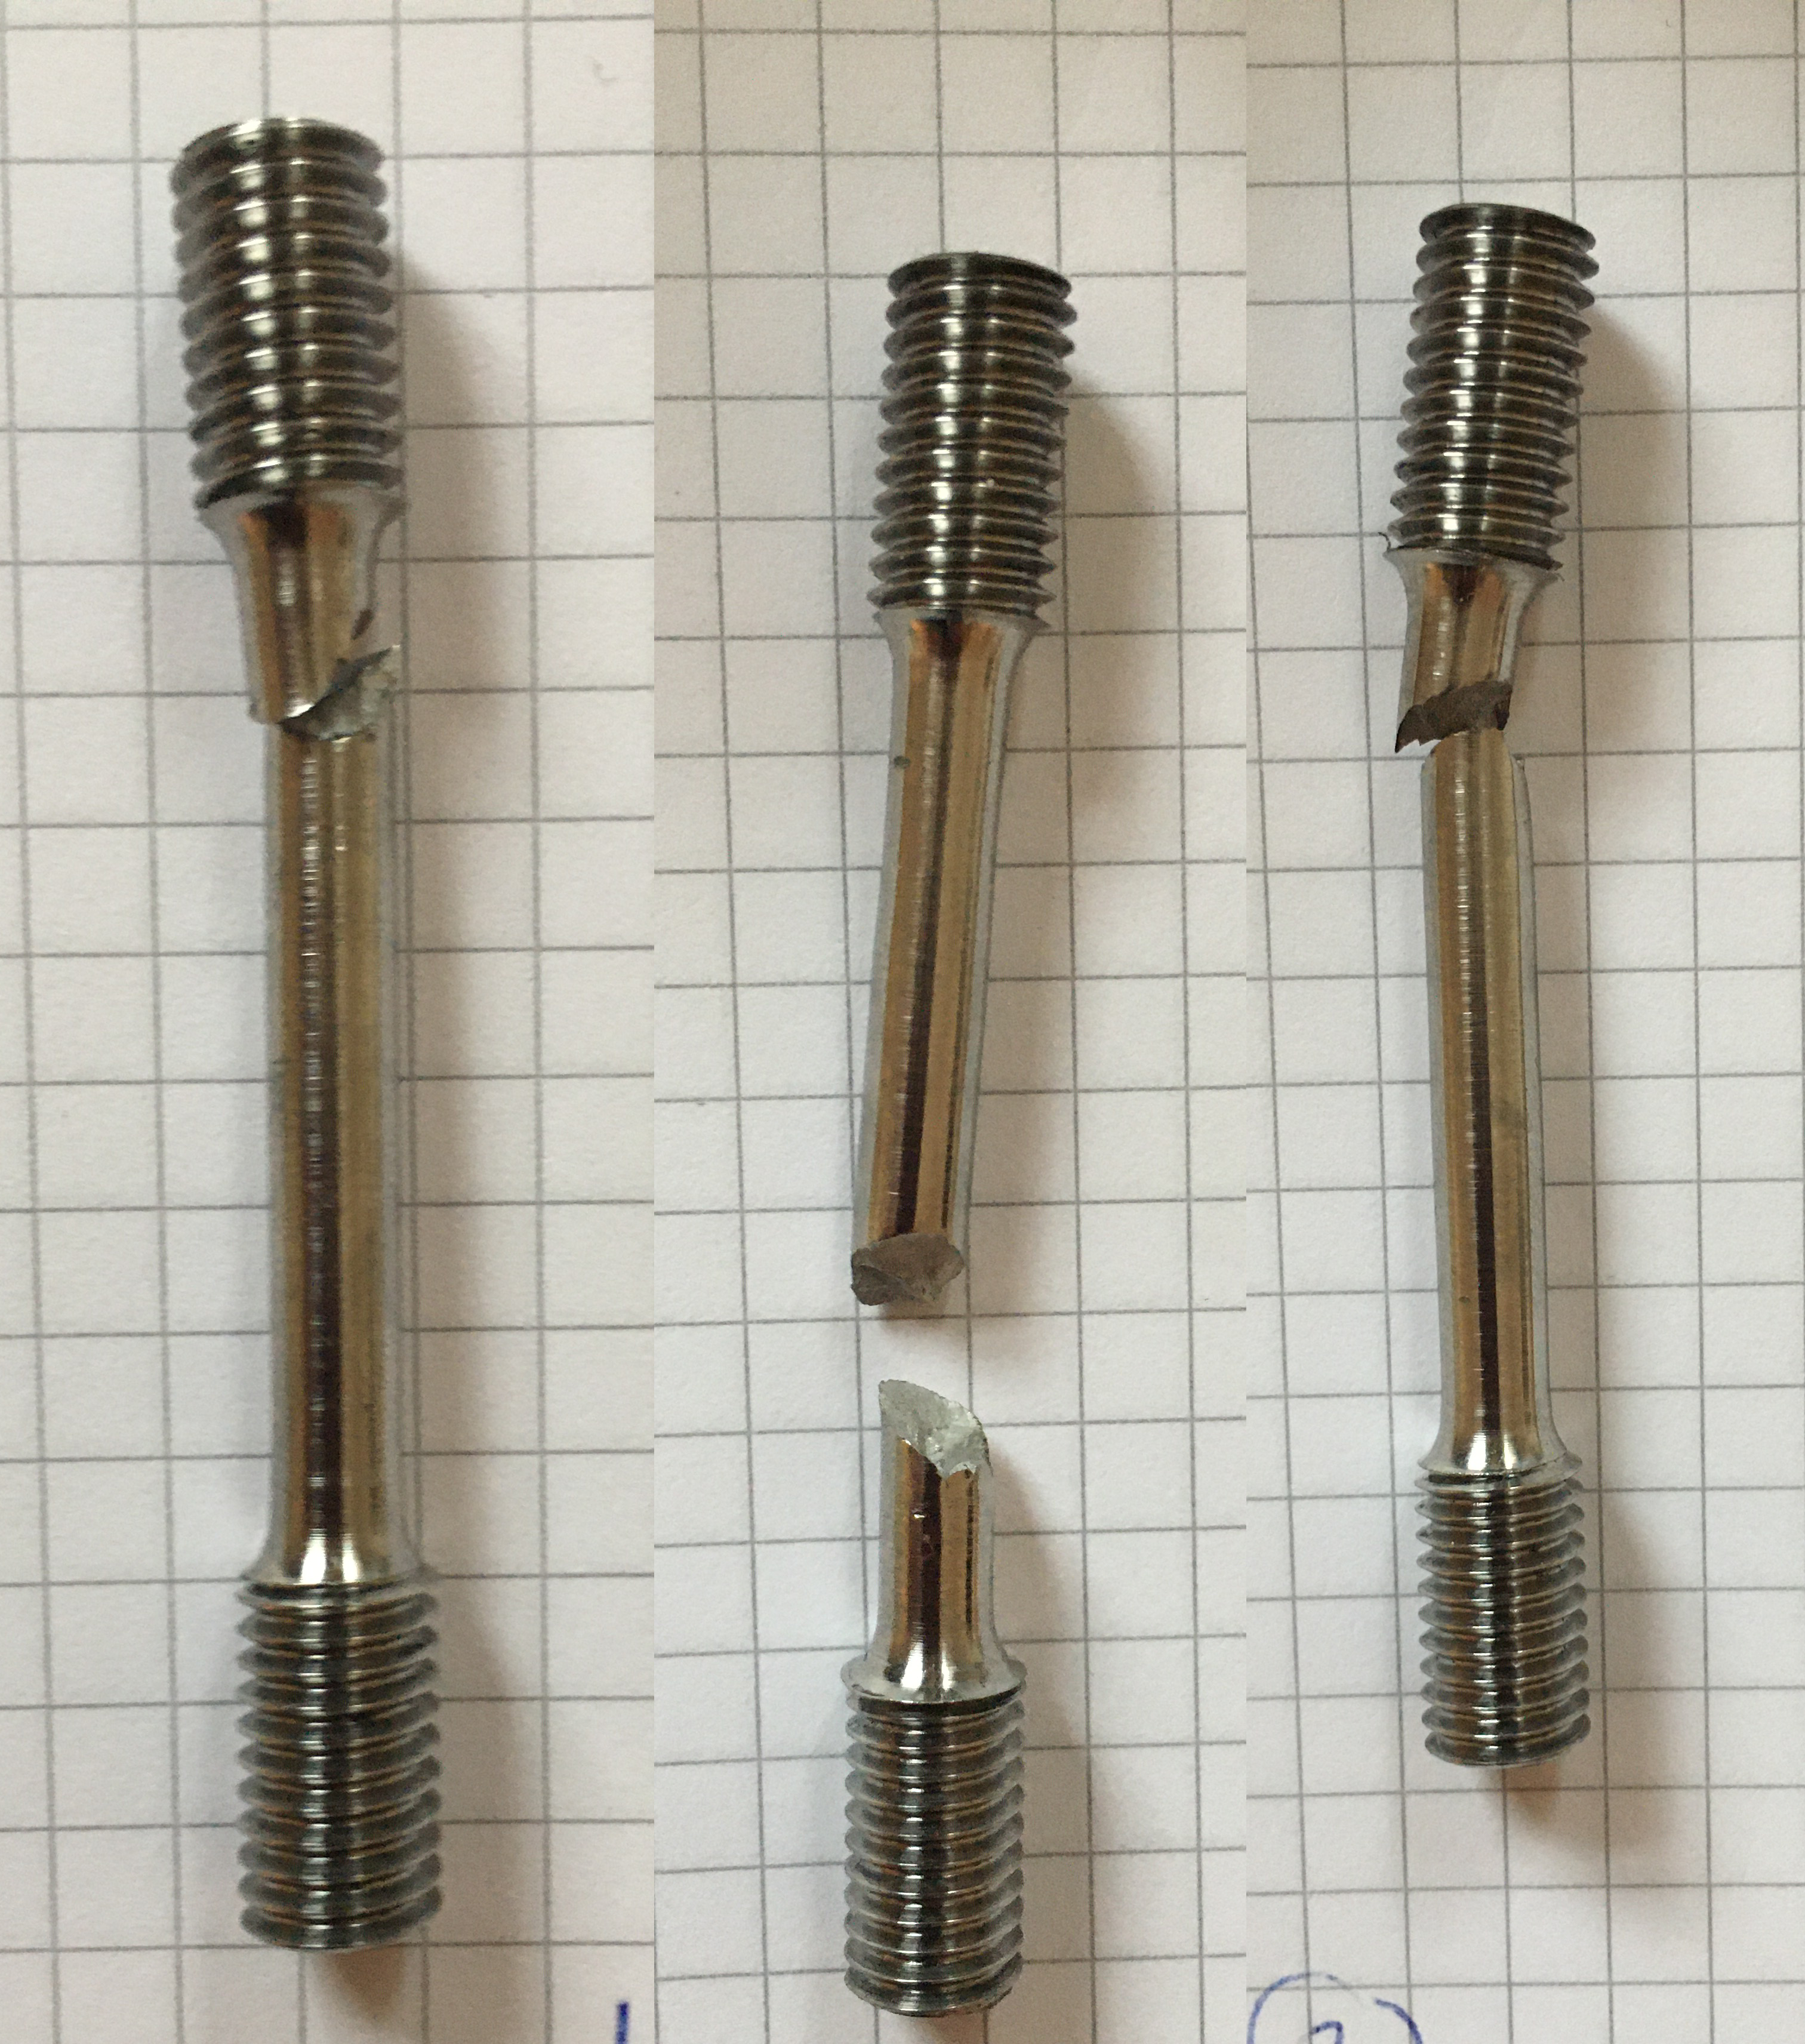
\includegraphics[width=0.6\linewidth]{./Bilder/Zugproben_kaputt}
	\caption{links: $\alpha_p + \alpha^\prime$-Probe, mitte und rechts: TS-STDA}
	\label{fig:zugkaputt}
\end{figure}

\begin{figure}
	\centering
	\includegraphics[width=0.8\linewidth]{./Bilder/Vergleich vor und nach Zerfall}
	\caption{Spannungs-Dehnungs-Diagramm für TS-STDA vor und nach dem Martensitzerfall}
	\label{fig:vergleich-vor-und-nach-zerfall}
\end{figure}

\begin{figure}
	\centering
	\includegraphics[width=0.8\linewidth]{./Bilder/Vergleich aller Proben}
	\caption{Spannungs-Dehnungs-Diagramm für alle Proben}
	\label{fig:vergleich-alle-proben}
\end{figure}

\begin{table}
	\centering
	\begin{tabular}{|c|c|c|c|c|c|c|c|}
		\hline
		Probe & $d_0$ [mm] & $S_0$ [mm$^2$] & \textit{E} [GPa] & $R_{p0,2}$ [MPa]& $R_m$ [MPa]& $A_g$ [\%]& $A$ [\%]\\
		\hline
		1 & 5,06 & 20,11 & 128 & 956 & 1019&4,8&17,9 \\
		\hline
		2 &5,04&19,95&122&946&1013&5,1&15,7\\
		\hline
		3 & 5,11&20,51& 122&1015&1085&2,1&3,0\\
		\hline
		4 &5,16& 20,91& 117 & 1007& 1090& 1,7&  1,9 \\
		\hline
		5&5,04 &19,95& 120& 952& 1033& 1,9 &2,5\\
		\hline
		6 &5,02& 19,79& 124& 968& 1023 &1,0 & 2,0\\
		\hline
		7&5,17& 20,99& 113& 925& 1042& 1,9& 2,1\\
		\hline
		8 & 5,12 & 20,59 & 118 & 952 & 1063 & 1,3 & 1,4\\
		\hline
	\end{tabular}
	\caption{Messwerte der Zugversuche bei 23,3$^\circ$C Raumtemperatur}
	\label{tab:zugversuche}
	
\end{table}

\pagebreak

\section{Diskussion der Ergebnisse (ZB)}

AR-Proben haben ein globulares Gefüge mit $\alpha$- und transformierter $\beta$-Phase (Abbildung \ref{fig:abbildung-8} a). Durch den großen Anteil an $\alpha_p$ konnten sich sehr feine $\alpha$-Lamellen in der transformierten $\beta$-Phase bilden, die für eine Duktilitätssteigerung sorgen. Aufgrund dieser feinen Strukturen haben AR-Proben eine relativ hohe Bruchdehnung \cite{Lutjering.2007}.

Die Proben 7 und 8 haben durch das Duplex-Glühen neben Martensit und kleinen $\alpha_p$-Körnern feine $\alpha$-Lamellen. Außerdem haben die Proben 5--8 im Vergleich zu den AR-Proben durch die Bildung von dünnen Martensitplatten feinere Gefügestrukturen. Dies führte vermutlich bei diesen Proben zu der Festigkeitszunahme. Das erklärt auch, dass Martensit, der nur eine beschränkte Duktiliät besitzt \cite{Lutjering.2007}, zu der niedrigen Duktilität dieser Proben geführt hat.\\
Des Weiteren hat die Probe 3 eine höhere Duktilität und Festigkeit gegenüber den Proben 7 und 8. Das kann durch den partiellen Martensit-Zerfall bzw. die Teiltransformation von $\alpha'$ in $\alpha$- und $\beta$-Phasen im letzten Schritt der Strategie 1 erklärt werden. Die Verfeinerung des Gefüges durch eine partielle Dekomposition der Martensitnadeln führt einerseits zu einer Steigerung der  Zugfestigkeit  und gleichzeitig zu einer Zunahme der Duktilität. 
Das bedeutet, dass ein weiterer Zerfall der Martensitstrukturen bei beiden Strategien zu einer Verbesserung der Bruchdehnung führen könnte. Dabei soll sich eine gröbere Gefügestruktur durch die Transformation von Martensit vollständig in $\alpha$- und $\beta$-Körner bilden. Dies ist möglich, wenn Proben aus Strategie 1 und 2 beim letzten Anlassen für längere Zeit bzw. bei höheren Temperaturen geglüht werden. Ein Beispiel für diese Optimierung der beiden Strategien zeigt die Tabelle \ref{wBZ}.



\begin{table}[h]
	\centering
	\begin{tabular}{|c|c|}
		\hline 
		Strategie & Wärmebehandlung \\ 
		\hline 
		1 & 983$^\circ$C/1h/AC + 950$^\circ$C/16$\pm $4min/WQ + 610$^\circ$C/1h/AC\\ 
		\hline 
		2 &  983$^\circ$C/1h/WQ + 800$^\circ$C/1.5--2h/AC \\ 
		\hline 
	\end{tabular} 
	\caption{Optimierungsbeispiele für Strategie 1 und 2}
	\label{wBZ}
	
	
\end{table}

Durch beide Strategien konnte eine Verfestigung von Ti-6242 erreicht werden. Die Dehngrenze hat dabei  die 10\% unterschritten. 
Aufgrund der kurzen Anlasszeiten und des starken Einflusses der Glühtemperatur auf die Gefügestruktur, ist die Reproduzierbarkeit der ersten Strategie für die Industrie ungenügend.














